% !TEX TS-program = pdflatex
\documentclass[aspectratio=169]{beamer}
\usepackage[utf8]{inputenc}
\usepackage[T1]{fontenc}
\usetheme{Madrid}
\usecolortheme{seahorse}
\usefonttheme{professionalfonts}
\setbeamertemplate{navigation symbols}{}
\setbeamercovered{transparent}
\setbeamertemplate{itemize items}[circle]
\setbeamertemplate{enumerate items}[default]
\setlength{\parskip}{0.15em}

\definecolor{bepurple}{RGB}{107,63,160}
\definecolor{begold}{RGB}{200,168,75}
\definecolor{beteal}{RGB}{26,122,110}
\definecolor{berust}{RGB}{192,68,42}
\definecolor{beblue}{RGB}{26,74,138}
\definecolor{softpurple}{RGB}{240,232,255}
\definecolor{softgold}{RGB}{255,248,220}
\definecolor{softteal}{RGB}{220,242,240}
\definecolor{softrust}{RGB}{255,235,230}
\setbeamercolor{structure}{fg=beblue}
\setbeamercolor{title}{fg=white,bg=beblue}
\setbeamercolor{frametitle}{fg=beblue}
% Minimal block rendering: regular/example blocks become colored headings (no box)
\setbeamertemplate{block begin}{%
  \par\vspace{0.2ex}%
  \ifx\insertblocktitle\empty\else%
    {\usebeamerfont{block title}\color{beblue}\textbf{\insertblocktitle}}\par\vspace{0.2ex}%
  \fi%
}
\setbeamertemplate{block end}{\par\vspace{0.2ex}}
\setbeamertemplate{block example begin}{%
  \par\vspace{0.2ex}%
  \ifx\insertblocktitle\empty\else%
    {\usebeamerfont{block title}\color{beteal}\textbf{\insertblocktitle}}\par\vspace{0.2ex}%
  \fi%
}
\setbeamertemplate{block example end}{\par\vspace{0.2ex}}
\setbeamertemplate{block alerted begin}{%
  \par\vspace{0.5ex}%
  \begin{beamercolorbox}[sep=0.5ex,rounded=true,shadow=false]{block title alerted}%
    \usebeamerfont{block title}\insertblocktitle%
  \end{beamercolorbox}%
  \nointerlineskip%
  \begin{beamercolorbox}[sep=0.5ex,rounded=true,shadow=false]{block body alerted}%
    \usebeamerfont{block body}%
}
\setbeamertemplate{block alerted end}{\end{beamercolorbox}\par\vspace{0.5ex}}
\setbeamercolor{block title alerted}{fg=white,bg=berust}
\setbeamercolor{block body alerted}{fg=black,bg=berust!8}
\setbeamercolor{alerted text}{fg=berust}

\usepackage{booktabs,amsmath,amssymb,array,multirow,hyperref,colortbl,xcolor}
\usepackage{tikz}
\usepackage{pgfplots}
\pgfplotsset{compat=1.18}
\usetikzlibrary{arrows.meta,positioning,calc,shapes.geometric,patterns}
\hypersetup{colorlinks=true,linkcolor=beblue,urlcolor=beblue}

\title{\textbf{Lecture 10: Applications and Policy Design}}
\subtitle{Bringing It All Together --- When, Where, and How Behavioural Economics Works}
\author{Prof.\ Muhebullah Karimzada}
\institute{School of Economics, University of Northern British Columbia}
\date{ECON 230 $\cdot$ Introduction to Behavioural Economics $\cdot$ Winter 2027}

\begin{document}

\begin{frame}[plain]\titlepage\end{frame}

% ============================================================
\begin{frame}{The Course in One Question}
\begin{alertblock}{The Central Question of Behavioural Policy}
\textbf{If people are systematically biased in predictable ways, what should policymakers do?}
\begin{enumerate}
  \item \textbf{Inform:} Tell people about their biases and let them correct themselves.
  \item \textbf{Incentivise:} Change prices and subsidies to align incentives.
  \item \textbf{Nudge:} Design the choice environment to exploit known biases for good.
  \item \textbf{Mandate:} Remove the choice entirely and impose the right outcome.
\end{enumerate}
\end{alertblock}
\begin{block}{Today's Lecture}
We apply the full toolbox of behavioural economics to four domains: \textbf{health}, \textbf{environment}, \textbf{finance}, and \textbf{tax compliance}. We also examine the \textbf{ethics and limits} of behavioural policy --- and assess the field's future.
\end{block}
\end{frame}

% ============================================================
\begin{frame}{The Policy Design Matrix}
\begin{center}\small
\begin{tabular}{p{1.8cm}p{3.2cm}p{3.2cm}p{2.8cm}}
\toprule
\textbf{Tool} & \textbf{Mechanism} & \textbf{When Best} & \textbf{Canadian Example}\\
\midrule
\textbf{Information} & Disclosure; education & When bias = lack of info & Calorie labels, FCAC\\
\textbf{Price/Tax} & Change financial incentive & High price elasticity & Carbon levy, cig.\ taxes\\
\rowcolor{softpurple}
\textbf{Nudge} & Defaults, framing, salience & Present bias / inertia & RRSP auto-enrol, organ donation\\
\textbf{Subsidy} & Reduce cost & Financial barrier binding & Canada Learning Bond\\
\textbf{Mandate} & Legal requirement & Large externalities & Helmet laws, car seats\\
\bottomrule
\end{tabular}
\end{center}
\begin{exampleblock}{Key Insight}
The tools complement each other. The best policy often \textit{combines} approaches --- a carbon levy (price) + awareness campaign (information) + green energy defaults (nudge).
\end{exampleblock}
\end{frame}

% ============================================================
\section{Health Policy}
% ============================================================

\begin{frame}{Behavioural Health Policy --- The Evidence}
Information campaigns alone are weak when the problem is present bias. 70\% of smokers \textit{know} smoking causes cancer.
\begin{columns}
\column{0.5\textwidth}
\begin{exampleblock}{What Works (RCT Evidence)}
\begin{itemize}\small
  \item \textbf{Commitment contracts:} Gym contracts $+$20\% attendance (Acland \& Levy, 2015).
  \item \textbf{Implementation intentions:} ``When/where will you get your shot?'' $\Rightarrow$ $+$13\% uptake.
  \item \textbf{Social norms:} ``Most patients take medication as prescribed'' $\Rightarrow$ $+$8\%.
\end{itemize}
\end{exampleblock}
\column{0.47\textwidth}
\begin{block}{Canada-Specific Successes}
\begin{itemize}\small
  \item \textbf{BC QuitNow:} 23\% quit rate vs 5\% unassisted.
  \item \textbf{Nova Scotia opt-out} (2021): registration rising.
  \item \textbf{BC CDC COVID messaging:} loss-framed prevention + gain-framed testing $\Rightarrow$ 2nd lowest mortality in Canada (2020).
\end{itemize}
\end{block}
\end{columns}
\end{frame}

% ============================================================
\begin{frame}{Vaccination: Why People Don't Vaccinate}
\begin{block}{Five Biases Working Against Vaccination}
{\small\begin{enumerate}[<+->]
  \item \textbf{Present bias:} Benefit (disease prevention) is future and uncertain; cost (going to clinic) is now and certain.
  \item \textbf{Optimism bias:} ``I won't get the flu.'' Overconfidence in own immunity --- a form of above-average effect.
  \item \textbf{Loss aversion:} Fear of side effects is \textit{salient and immediate}; disease prevention is \textit{abstract and future}.
  \item \textbf{Availability heuristic:} If nobody in your social network got the flu last year, perceived risk is low.
  \item \textbf{Descriptive social norms:} If peers don't vaccinate, the descriptive norm actively discourages vaccination.
\end{enumerate}}
\end{block}
\pause
\begin{alertblock}{Key Insight}
\small The problem is \textbf{not lack of information} --- 70\%+ of Canadians know vaccines work. It is a collection of biases pulling in the opposite direction.
\end{alertblock}
\end{frame}

% ============================================================
\begin{frame}{Vaccination: Behavioural Solutions (RCT Evidence)}
\begin{exampleblock}{Milkman et al.\ (2021) --- 47,000-Person RCT at a US Health System}
\begin{itemize}
  \item \textbf{Reminder only:} $+$4\% uptake vs control.
  \item \textbf{Reminder + Implementation Intention} (``When/where will you go?''): $+$13\% uptake.
  \item \textbf{Ownership frame} (``Your flu shot is waiting for you''): $+$11\% uptake.
  \item \textbf{Reminder + pre-booked appointment:} $+$15\% uptake.
  \item \textbf{Cost of all interventions: \$0.} (Only wording on a text message.)
\end{itemize}
\end{exampleblock}
\begin{block}{Canadian Applications}
\begin{itemize}
  \item \textbf{COVID-19 messaging (BC CDC, 2020):} Loss-framed prevention messages + gain-framed testing messages $\Rightarrow$ 2nd lowest mortality rate in Canada.
  \item \textbf{BC Pharmacare flu programme:} Text reminder with ``your shot is available at [pharmacy name]'' $\Rightarrow$ 18\% uptake increase (2022 pilot).
\end{itemize}
\end{block}
\end{frame}

% ============================================================
\section{Environment}
% ============================================================

\begin{frame}{Behavioural Environmental Policy}
Standard tools face limits: carbon taxes face loss-aversion resistance; subsidies are costly; cap-and-trade is complex.
\begin{columns}
\column{0.5\textwidth}
\begin{exampleblock}{Behavioural Tools}
\begin{itemize}\small
  \item \textbf{Social norms:} Opower reports $\Rightarrow$ 2\% reduction $=$ 1 power plant per 6M users.
  \item \textbf{Green default:} 69\% opt-out vs 7\% opt-in.
  \item \textbf{Commitment:} BC Hydro Team Power Smart $\Rightarrow$ 10\%+ reduction.
  \item \textbf{Salience:} Real-time CO$_2$ on Nest/Ecobee.
\end{itemize}
\end{exampleblock}
\column{0.47\textwidth}
\begin{alertblock}{BC Case Study}
BC carbon tax (2008): revenue-neutral framing + gain frame for rebates + explicit per-household calculation $\Rightarrow$ became \textbf{broadly popular}. Lesson: \textit{frame determines political feasibility.}
\end{alertblock}
\end{columns}
\end{frame}

% ============================================================
\begin{frame}{Food Choices and Behavioural Policy}
\textcolor{beblue}{\textbf{Three Approaches: Meat Consumption Reduction}}
\begin{center}\small
\begin{tabular}{lp{4cm}l}
\toprule
\textbf{Approach} & \textbf{Intervention} & \textbf{Effect}\\
\midrule
Information & Pamphlet on environmental cost of meat & 2\% reduction\\
Price & 20\% meat tax & 7\% reduction\\
\rowcolor{softpurple}
Nudge (default) & Plant-based option as canteen default & \textbf{15\% reduction}\\
Nudge (salience) & Green leaf label on plant-based items & 5\% reduction\\
Mandate & No meat options at all & 100\% (backlash risk)\\
\bottomrule
\end{tabular}
\end{center}
\begin{exampleblock}{Denmark Case Study}
Danish hospitals set plant-based food as the default in staff canteens (2013). Plant-based consumption rose \textbf{400\%}. Zero complaints. Food waste fell 35\%. Canadian hospital food service: similar pilots proposed for BC hospital cafeterias (2023 proposal to BC Ministry of Health).
\end{exampleblock}
\end{frame}

% ============================================================
\section{Financial Policy}
% ============================================================

\begin{frame}{Behavioural Financial Regulation}
\textbf{Canadian regulators:} FCAC (fee disclosure, min-payment warnings) $\cdot$ OSFI (mortgage stress testing B-20, 2018 --- commitment device) $\cdot$ CIPF (investment dealer disclosure).
\begin{columns}
\column{0.5\textwidth}
\begin{alertblock}{Key Principles}
\begin{enumerate}\small
  \item \textbf{Salience:} One-page ``Key Facts'' for mortgages (2022).
  \item \textbf{Defaults:} Auto-enrollment over mandates.
  \item \textbf{Friction reduction:} CRA pre-fill.
  \item \textbf{Sludge removal:} Easy cancellation.
\end{enumerate}
\end{alertblock}
\column{0.47\textwidth}
\begin{exampleblock}{CRM2 Reforms (2016)}
Required disclosure of (1) fees in dollars; (2) performance vs benchmark. Fee awareness soared. Shift to ETFs accelerated: Canadian ETF AUM \$80B (2016) $\to$ \textbf{\$350B} (2023).
\end{exampleblock}
\end{columns}
\end{frame}

% ============================================================
\begin{frame}{Tax Compliance --- Behavioural Approach}
\begin{block}{Why People Don't Pay Their Taxes (Behavioural Perspective)}
\begin{itemize}
  \item \textbf{Present bias:} Payment is now; enforcement is uncertain and future.
  \item \textbf{Social norms:} If you believe others are evading, social constraint is relaxed.
  \item \textbf{Complexity:} Cognitive overload from complex forms $\Rightarrow$ errors and avoidance.
  \item \textbf{Loss aversion:} A tax payment is experienced as a loss (even though taxes are obligations).
\end{itemize}
\end{block}
\begin{exampleblock}{The BIT's HMRC Experiments (UK Tax Authority)}
\begin{itemize}
  \item Adding social norm: $+$15\% payment rate.
  \item Simplifying the letter: $+$5\% payment rate.
  \item Adding implementation intention: ``Pay online in 3 minutes at hmrc.gov.uk/pay'' $\Rightarrow$ $+$8\%.
  \item Combined: \textbf{$+$28\%} vs standard letter. Revenue impact: hundreds of millions of pounds.
  \item CRA adoption of similar strategies: $+$\$200M estimated annual revenue at full scale.
\end{itemize}
\end{exampleblock}
\end{frame}

% ============================================================
\section{Ethics and Limits}
% ============================================================

\begin{frame}{Criticisms of Nudges --- A Fair Assessment}
\begin{columns}
\column{0.5\textwidth}
\begin{alertblock}{The Criticisms}
\begin{enumerate}\small
  \item \textbf{Manipulation:} Exploiting biases vs helping people reason better.
  \item \textbf{Autonomy:} Infringes self-determination.
  \item \textbf{Paternalism:} Who decides? Government can be wrong.
  \item \textbf{Scale:} Small effects; systemic problems need systemic solutions.
  \item \textbf{Corruption:} Corporations use same techniques against consumers.
\end{enumerate}
\end{alertblock}
\column{0.47\textwidth}
\begin{block}{The Defenders' Response}
\begin{enumerate}\small
  \item Transparency + opt-out = legitimate.
  \item Someone always designs the environment.
  \item Paternalism can be evaluated and reversed.
  \item Small effects $\times$ scale = large aggregate benefit.
  \item Regulate corporate nudges separately.
\end{enumerate}
\end{block}
\end{columns}
\textcolor{beteal}{\textbf{Thaler (2018):}} Nudges are ethical when transparent, opt-outable, evidence-based, and benefit the chooser.
\end{frame}

% ============================================================
\begin{frame}{When Do Nudges Fail?}
\begin{block}{Limits of the Nudge Approach}
\begin{enumerate}[<+->]
  \item \textbf{Structural vs behavioural problems:} If people can't save because wages are too low, a default doesn't help. Nudges work within a given constraint set --- they don't change the constraints.
  \item \textbf{Effect size:} Many nudge effects are statistically significant but economically small (1--3\%). Systemic health or environmental challenges require larger interventions.
  \item \textbf{Persistence:} Some nudge effects fade over time. Auto-enrollment raises participation but not always contribution rates.
  \item \textbf{Heterogeneity:} One default cannot fit all. Personalised nudges are more effective but harder to implement at scale.
  \item \textbf{Adaptation:} Sophisticated individuals (often higher-income) learn to ignore or reverse nudges. This can make nudges regressive.
\end{enumerate}
\end{block}
\end{frame}

% ============================================================
\begin{frame}{The Welfare Question}
With time-inconsistent preferences, there are \textbf{three} selves: \textbf{Instant} ($\beta<1$: wants cake now); \textbf{Long-run} ($\beta=1$: wants health); \textbf{Reflective} (may endorse either).
\begin{exampleblock}{O'Donoghue \& Rabin (2003)}
Paternalistic correction of present bias is welfare-improving if the long-run preference is the ``true'' preference --- not always clear for addiction and lifestyle choices.
\end{exampleblock}
\begin{alertblock}{The Libertarian Critique (Sugden, 2017)}
Even if people are biased, it doesn't follow that government knows better. Governments have their own biases and political incentives. Behavioural policy could become a tool for political manipulation.
\end{alertblock}
\end{frame}

% ============================================================
\begin{frame}{[GAME] Policy Design Challenge}
\note{Final in-class exercise. Groups design a complete behavioural policy intervention. Present and critique each other. This integrates all 10 lectures.}
\begin{alertblock}{Final Group Challenge --- 8 Minutes}
Canada's federal government asks you to design a behavioural policy intervention for one problem:
\begin{itemize}
  \item \textbf{Group A:} Increase RRSP contributions among 25--40 year olds.
  \item \textbf{Group B:} Reduce single-use plastic in university cafeterias.
  \item \textbf{Group C:} Increase workplace vaccination rates to 90\%+.
  \item \textbf{Group D:} Reduce payday loan usage in low-income communities.
\end{itemize}
Your intervention must: (1) identify the key bias, (2) propose one nudge and one complementary intervention, (3) describe your RCT evaluation design.
\end{alertblock}
\end{frame}

% ============================================================
\begin{frame}{The Future of Behavioural Economics}
\begin{block}{Emerging Frontiers}
\begin{enumerate}
  \item \textbf{Personalised nudges:} Machine learning to match nudge to individual bias profile. Amazon, Spotify already do this commercially.
  \item \textbf{Neuroeconomics:} fMRI identifies neural mechanisms; predicts who responds to which nudge.
  \item \textbf{Digital nudges:} Notifications, app design, smart defaults. The smartphone is the greatest nudge delivery platform ever invented.
  \item \textbf{International development:} JPAL (Banerjee, Duflo) applies behavioural tools in low-income countries. Nobel Prize 2019.
  \item \textbf{Climate change:} Behavioural public economics integrated with climate policy. Paris Agreement pledges: present-biased governments.
\end{enumerate}
\end{block}
\begin{exampleblock}{The Reproducibility Debate}
Camerer et al.\ (2018): 61\% of 18 replication attempts of lab results succeeded. Loss aversion, present bias, anchoring: \textbf{high replication}. Some social priming effects: \textbf{failed}. Lesson: policy should rely on highly replicated findings.
\end{exampleblock}
\end{frame}

% ============================================================
\begin{frame}{The Course in One Diagram}
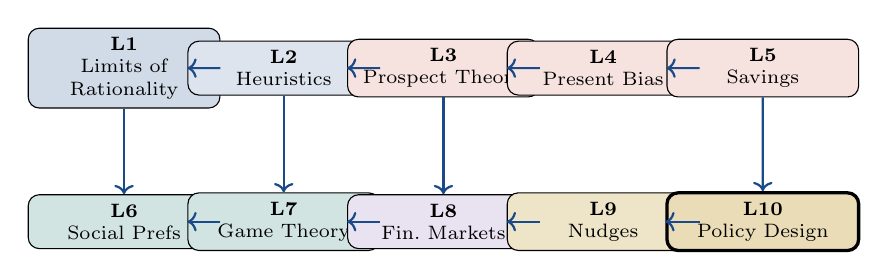
\begin{tikzpicture}[scale=0.78]
\node[draw,fill=beblue!20,rounded corners,text width=2.2cm,align=center,font=\scriptsize] (L1) at (0,4) {\textbf{L1}\\ Limits of Rationality};
\node[draw,fill=beblue!15,rounded corners,text width=2.2cm,align=center,font=\scriptsize] (L2) at (2.6,4) {\textbf{L2}\\ Heuristics};
\node[draw,fill=berust!15,rounded corners,text width=2.2cm,align=center,font=\scriptsize] (L3) at (5.2,4) {\textbf{L3}\\ Prospect Theory};
\node[draw,fill=berust!15,rounded corners,text width=2.2cm,align=center,font=\scriptsize] (L4) at (7.8,4) {\textbf{L4}\\ Present Bias};
\node[draw,fill=berust!15,rounded corners,text width=2.2cm,align=center,font=\scriptsize] (L5) at (10.4,4) {\textbf{L5}\\ Savings};
\node[draw,fill=beteal!20,rounded corners,text width=2.2cm,align=center,font=\scriptsize] (L6) at (0,1.5) {\textbf{L6}\\ Social Prefs};
\node[draw,fill=beteal!20,rounded corners,text width=2.2cm,align=center,font=\scriptsize] (L7) at (2.6,1.5) {\textbf{L7}\\ Game Theory};
\node[draw,fill=bepurple!15,rounded corners,text width=2.2cm,align=center,font=\scriptsize] (L8) at (5.2,1.5) {\textbf{L8}\\ Fin.\ Markets};
\node[draw,fill=begold!30,rounded corners,text width=2.2cm,align=center,font=\scriptsize] (L9) at (7.8,1.5) {\textbf{L9}\\ Nudges};
\node[draw,fill=begold!40,rounded corners,text width=2.2cm,align=center,font=\scriptsize,very thick] (L10) at (10.4,1.5) {\textbf{L10}\\ Policy Design};
\foreach \from/\to in {L1/L2,L2/L3,L3/L4,L4/L5,L6/L7,L7/L8,L8/L9,L9/L10}{
  \draw[->,thick,beblue] (\from) -- (\to);}
\draw[->,thick,beblue] (L1) -- (L6);
\draw[->,thick,beblue] (L2) -- (L7);
\draw[->,thick,beblue] (L3) -- (L8);
\draw[->,thick,beblue] (L5) -- (L10);
\end{tikzpicture}
\medskip
\begin{block}{\centering The Core Message}
\centering\textit{``People are not irrational. They are intentionally rational --- but cognitively constrained. Understanding those constraints is how we build a better world.''}
\end{block}
\end{frame}

% ============================================================
\begin{frame}{Final Exam and Assessment Reminders}
\begin{block}{What You Should Be Able to Do}
\begin{itemize}
  \item \textbf{Identify} which bias is operating in a given real-world situation.
  \item \textbf{Predict} how a present-biased, loss-averse, overconfident agent would behave.
  \item \textbf{Design} a nudge that addresses a specific behavioural failure --- with justification.
  \item \textbf{Evaluate} a policy using cost-benefit analysis that accounts for behavioural responses.
  \item \textbf{Critique} nudge-based policy using autonomy, effectiveness, and distributive arguments.
  \item \textbf{Apply} Canadian data and context to global behavioural economic findings.
\end{itemize}
\end{block}
\begin{alertblock}{One Last Thought}
Behavioural economics does not replace standard economics. It \textit{enriches} it. The standard model tells you what perfectly rational agents would do --- the ideal benchmark. Behavioural economics tells you what real people actually do --- and how to close the gap. Together, they are the most powerful toolkit in modern social science.
\end{alertblock}
\end{frame}

% ============================================================
\begin{frame}{Key Takeaways --- Lecture 10 \& The Course}
\begin{itemize}
  \item[\textcolor{beteal}{\checkmark}] \textbf{Policy toolkit:} information, price, nudge, subsidy, mandate --- different tools for different biases.
  \item[\textcolor{beteal}{\checkmark}] \textbf{Health policy:} implementation intentions, commitment contracts, and loss framing outperform information campaigns alone.
  \item[\textcolor{beteal}{\checkmark}] \textbf{Environmental policy:} green energy defaults, social norms, and carbon levy framing.
  \item[\textcolor{beteal}{\checkmark}] \textbf{Financial regulation:} salience, friction reduction, sludge removal, CRM2 disclosure.
  \item[\textcolor{beteal}{\checkmark}] \textbf{Tax compliance:} social norms + simplification = hundreds of millions in additional revenue.
  \item[\textcolor{beteal}{\checkmark}] \textbf{Ethics:} nudges are legitimate when transparent, easy to opt out, evidence-based, and benefit the chooser.
  \item[\textcolor{beteal}{\checkmark}] \textbf{Limits:} nudges don't fix structural problems; effects can be small; personalisation needed.
\end{itemize}
\medskip
\centering \textit{``The best way to make the world a better place is not to tell people what to do --- but to understand why they do what they do.''}\\
\small --- Behavioural Economics, ECON 230, UNBC, Winter 2027
\end{frame}

% ============================================================
\begin{frame}{Course Bibliography --- Key References}
\footnotesize
\begin{columns}
\column{0.5\textwidth}
\textbf{Foundations}\\
Kahneman (2011). \textit{Thinking, Fast and Slow.}\\
Simon (1955). \textit{QJE}: Bounded rationality.\\
Tversky \& Kahneman (1974). \textit{Science}: Heuristics.\\[0.3em]
\textbf{Prospect Theory}\\
Kahneman \& Tversky (1979). \textit{Econometrica}.\\
Tversky \& Kahneman (1992). \textit{J. Risk \& Uncertainty}.\\[0.3em]
\textbf{Time}\\
Laibson (1997). \textit{QJE}: Golden eggs.\\
O'Donoghue \& Rabin (1999). \textit{AER}.\\
Thaler \& Benartzi (2004). \textit{JPE}: SMarT.\\[0.3em]
\textbf{Social Preferences}\\
Fehr \& Schmidt (1999). \textit{QJE}: Inequality aversion.\\
Fehr \& Gächter (2002). \textit{Nature}: Altruistic punishment.
\column{0.47\textwidth}
\textbf{Game Theory}\\
Camerer (2003). \textit{Behavioral Game Theory}.\\
Nagel (1995). \textit{AER}: Beauty contest.\\[0.3em]
\textbf{Finance}\\
Odean (1998). \textit{J. Finance}: Disposition.\\
DeLong et al. (1990). \textit{JPE}: Noise traders.\\
Shleifer \& Vishny (1997). \textit{J. Finance}: Limits.\\[0.3em]
\textbf{Nudges \& Policy}\\
Thaler \& Sunstein (2008). \textit{Nudge.}\\
Madrian \& Shea (2001). \textit{QJE}: Auto-enrollment.\\
Allcott (2011). \textit{J.\ Public Econ}: Opower.\\
BIT (2012). \textit{Applying Behavioural Insights.}\\
Impact Canada (2020). \textit{Annual Evaluation Report.}
\end{columns}
\end{frame}

\end{document}
